\tikzset{every picture/.style={line width=0.75pt}} %set default line width to 0.75pt        
\noindent
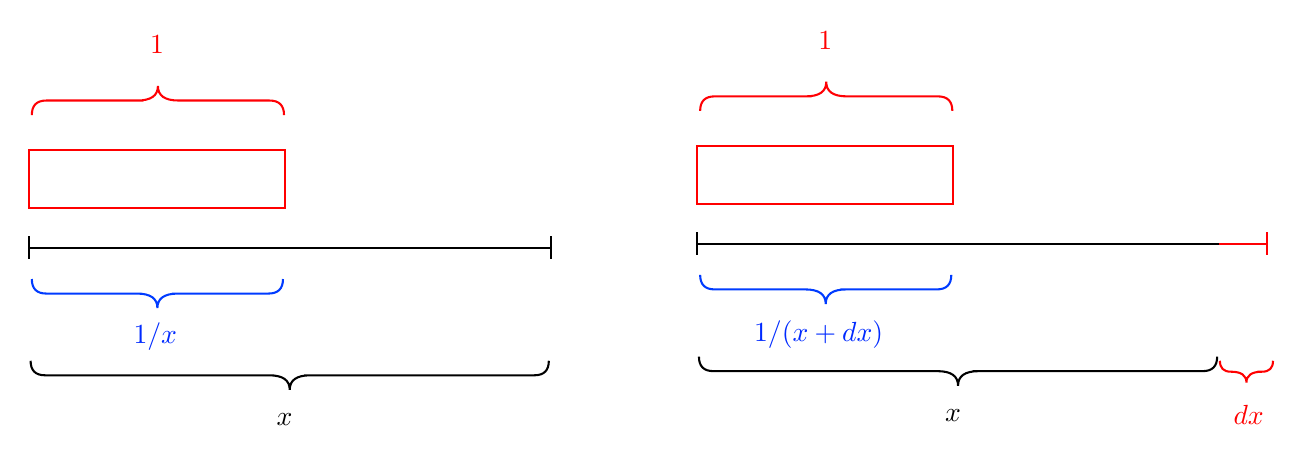
\begin{tikzpicture}[x=0.75pt,y=0.75pt,yscale=-1,xscale=1]
%uncomment if require: \path (0,300); %set diagram left start at 0, and has height of 300

%Straight Lines [id:da21843410649174944] 
\draw    (26,152) -- (277.5,152) ;
\draw [shift={(277.5,152)}, rotate = 180] [color={rgb, 255:red, 0; green, 0; blue, 0 }  ][line width=0.75]    (0,5.59) -- (0,-5.59)   ;
\draw [shift={(26,152)}, rotate = 180] [color={rgb, 255:red, 0; green, 0; blue, 0 }  ][line width=0.75]    (0,5.59) -- (0,-5.59)   ;
%Shape: Rectangle [id:dp4515994731638744] 
\draw  [color={rgb, 255:red, 255; green, 0; blue, 0 }  ,draw opacity=1 ] (26,105) -- (149.5,105) -- (149.5,133) -- (26,133) -- cycle ;
%Shape: Brace [id:dp08423244109966566] 
\draw  [color={rgb, 255:red, 0; green, 0; blue, 0 }  ,draw opacity=1 ] (26.91,206.38) .. controls (26.91,211.05) and (29.24,213.38) .. (33.91,213.38) -- (141.75,213.38) .. controls (148.42,213.38) and (151.75,215.71) .. (151.75,220.38) .. controls (151.75,215.71) and (155.08,213.38) .. (161.75,213.38)(158.75,213.38) -- (269.59,213.38) .. controls (274.26,213.38) and (276.59,211.05) .. (276.59,206.38) ;
%Shape: Brace [id:dp03278570786281365] 
\draw  [color={rgb, 255:red, 255; green, 0; blue, 4 }  ,draw opacity=1 ] (149,88) .. controls (149,83.33) and (146.67,81) .. (142,81) -- (98.25,81) .. controls (91.58,81) and (88.25,78.67) .. (88.25,74) .. controls (88.25,78.67) and (84.92,81) .. (78.25,81)(81.25,81) -- (34.5,81) .. controls (29.83,81) and (27.5,83.33) .. (27.5,88) ;
%Shape: Brace [id:dp9522391936570531] 
\draw  [color={rgb, 255:red, 0; green, 59; blue, 255 }  ,draw opacity=1 ] (27.5,167) .. controls (27.5,171.67) and (29.83,174) .. (34.5,174) -- (78,174) .. controls (84.67,174) and (88,176.33) .. (88,181) .. controls (88,176.33) and (91.33,174) .. (98,174)(95,174) -- (141.5,174) .. controls (146.17,174) and (148.5,171.67) .. (148.5,167) ;
%Straight Lines [id:da4718568555643836] 
\draw    (348,150) -- (599.5,150) ;
\draw [shift={(348,150)}, rotate = 180] [color={rgb, 255:red, 0; green, 0; blue, 0 }  ][line width=0.75]    (0,5.59) -- (0,-5.59)   ;
%Shape: Rectangle [id:dp8513478800250758] 
\draw  [color={rgb, 255:red, 255; green, 0; blue, 0 }  ,draw opacity=1 ] (348,103) -- (471.5,103) -- (471.5,131) -- (348,131) -- cycle ;
%Shape: Brace [id:dp17739490270334712] 
\draw  [color={rgb, 255:red, 0; green, 0; blue, 0 }  ,draw opacity=1 ] (348.91,204.38) .. controls (348.91,209.05) and (351.24,211.38) .. (355.91,211.38) -- (463.75,211.38) .. controls (470.42,211.38) and (473.75,213.71) .. (473.75,218.38) .. controls (473.75,213.71) and (477.08,211.38) .. (483.75,211.38)(480.75,211.38) -- (591.59,211.38) .. controls (596.26,211.38) and (598.59,209.05) .. (598.59,204.38) ;
%Shape: Brace [id:dp9740788101727171] 
\draw  [color={rgb, 255:red, 255; green, 0; blue, 4 }  ,draw opacity=1 ] (471,86) .. controls (471,81.33) and (468.67,79) .. (464,79) -- (420.25,79) .. controls (413.58,79) and (410.25,76.67) .. (410.25,72) .. controls (410.25,76.67) and (406.92,79) .. (400.25,79)(403.25,79) -- (356.5,79) .. controls (351.83,79) and (349.5,81.33) .. (349.5,86) ;
%Shape: Brace [id:dp5640321305233592] 
\draw  [color={rgb, 255:red, 0; green, 59; blue, 255 }  ,draw opacity=1 ] (349.5,165) .. controls (349.5,169.67) and (351.83,172) .. (356.5,172) -- (400,172) .. controls (406.67,172) and (410,174.33) .. (410,179) .. controls (410,174.33) and (413.33,172) .. (420,172)(417,172) -- (463.5,172) .. controls (468.17,172) and (470.5,169.67) .. (470.5,165) ;
%Shape: Brace [id:dp5650547309026009] 
\draw  [color={rgb, 255:red, 255; green, 0; blue, 0 }  ,draw opacity=1 ] (599.91,206.38) .. controls (599.91,209.89) and (601.67,211.65) .. (605.18,211.65) -- (605.18,211.65) .. controls (610.19,211.65) and (612.7,213.41) .. (612.7,216.92) .. controls (612.7,213.41) and (615.21,211.65) .. (620.23,211.65)(617.97,211.65) -- (620.23,211.65) .. controls (623.74,211.65) and (625.5,209.89) .. (625.5,206.38) ;
%Straight Lines [id:da6965968095386313] 
\draw [color={rgb, 255:red, 255; green, 0; blue, 4 }  ,draw opacity=1 ]   (599.5,150) -- (622.5,150)  ;
\draw [shift={(622.5,150)}, rotate = 180] [color={rgb, 255:red, 255; green, 0; blue, 4 }  ,draw opacity=1 ][line width=0.75]    (0,5.59) -- (0,-5.59)   ;

% Text Node
\draw (144,230.4) node [anchor=north west][inner sep=0.75pt]    {$x$};
% Text Node
\draw (83,48.4) node [anchor=north west][inner sep=0.75pt]  [color={rgb, 255:red, 255; green, 0; blue, 0 }  ,opacity=1 ]  {$1$};
% Text Node
\draw (75,186.4) node [anchor=north west][inner sep=0.75pt]  [color={rgb, 255:red, 0; green, 42; blue, 255 }  ,opacity=1 ]  {$1/x$};
% Text Node
\draw (466,228.4) node [anchor=north west][inner sep=0.75pt]    {$x$};
% Text Node
\draw (405,46.4) node [anchor=north west][inner sep=0.75pt]  [color={rgb, 255:red, 255; green, 0; blue, 0 }  ,opacity=1 ]  {$1$};
% Text Node
\draw (374,185.4) node [anchor=north west][inner sep=0.75pt]  [color={rgb, 255:red, 0; green, 42; blue, 255 }  ,opacity=1 ]  {$1/( x+dx)$};
% Text Node
\draw (605,226.4) node [anchor=north west][inner sep=0.75pt]  [color={rgb, 255:red, 255; green, 0; blue, 0 }  ,opacity=1 ]  {$dx$};


\end{tikzpicture}